\documentclass[
  12pt, % Fontsize
  a4paper, % papersize
  twoside, % For twosided documents
  openany, % Chapters start always at a odd page
  numbers=noenddot, % No final dots in Sectionnumbers, e.g 1.2 instead of 1.2.
  BCOR=5mm, % Correction length for lost space from binding
  parskip=half*, %No indent but spacing between paragraphs
  thesis, % type of document
]{bfhbook}


% Test Template for bfhbook.cls
\usepackage[T1]{fontenc}
% Coding 
\usepackage[utf8]{inputenc}
% Language setting
\usepackage[german]{babel}
\usepackage[export]{adjustbox}

% \usepackage{fonttable}
% Hyperref
\usepackage[                
  pdftex,                  % for PDF
  colorlinks=true,         % colored links
  linkcolor=black,         % color for links
  citecolor=black,         % color for references
  urlcolor=black,          % color for url 
  bookmarks=true
]{hyperref}              

\usepackage{booktabs} % For nicer tables
\usepackage{threeparttable} % Table-Captions having the same width than the table
\usepackage[singlelinecheck=off]{caption}
\usepackage{siunitx} % Scientific Units and number setting
\usepackage{listings} % For Program-Code
\usepackage{minted}[frame=single,
               framesep=3mm,
               linenos=true,
               xleftmargin=21pt,
               tabsize=4,
               breaklines]

\usepackage{caption}
\captionsetup[figure]{font=footnotesize, labelfont=small}
\newcommand{\source}[1]{\caption*{Quelle: {#1}} }

\usepackage{xcolor}

\usepackage[export]{adjustbox}
\usepackage[document]{ragged2e} % left-alignment for text

\usepackage{glossaries}

% definition for directory tree with forest
\usepackage[edges]{forest}

\definecolor{foldercolor}{RGB}{124,166,198}

\tikzset{pics/folder/.style={code={%
    \node[inner sep=0pt, minimum size=#1](-foldericon){};
    \node[folder style, inner sep=0pt, minimum width=0.3*#1, minimum height=0.6*#1, above right, xshift=0.05*#1] at (-foldericon.west){};
    \node[folder style, inner sep=0pt, minimum size=#1] at (-foldericon.center){};}
    },
    pics/folder/.default={20pt},
    folder style/.style={draw=foldercolor!80!black,top color=foldercolor!40,bottom color=foldercolor}
}

\forestset{is file/.style={edge path'/.expanded={%
        ([xshift=\forestregister{folder indent}]!u.parent anchor) |- (.child anchor)},
        inner sep=1pt},
    this folder size/.style={edge path'/.expanded={%
        ([xshift=\forestregister{folder indent}]!u.parent anchor) |- (.child anchor) pic[solid]{folder=#1}}, inner xsep=0.6*#1},
    folder tree indent/.style={before computing xy={l=#1}},
    folder icons/.style={folder, this folder size=#1, folder tree indent=3*#1},
    folder icons/.default={12pt},
}

% end definition directory tree

%%%%%%%%%%%%%%%%%%%%%%%%%%%%%%%%%%%
% Settings 
%%%%%%%%%%%%%%%%%%%%%%%%%%%%%%%%
% Type?? (Lecture Notes, BSc Thesis, Master Thesis, . . .) 
% Use Variables \BSc, \Master, etc. for language support
\type{Semesterarbeit}
% Author(s)
\author{Marc Habegger}
% Title
\title{IoT Erfassung von und Darstellung Sensordaten}
% Short Title, will be used in the footline
\shorttitle{CAS BGD Semesterarbeit}
% Subtitle
\subtitle{CAS Big Data}
% Titlepicture
\titlepicture{Bilder/Titel.png}
%%

% Topic of Study
\degreeprogramme{CAS Big Data}
% Expert
\expert{Max Kleiner}
% Version
\version{1.0}
% Date
\date{\today} % Or any other possible date

% Departement
% Use Variable for language support
%\TI

% Semester
% Use Variable for language support
%\semester

% Logo(s)

% Colors
% Secondary Color for Graphics, Tables etc.
% Naming: BFH*Color*light|middle|dark, e.g. BFHGreendark, BFHBluelight, etc.
% Possible Color Values: Green, Blue, Purple, Brown 
\newcommand{\seccolor}{BFHLightGreen} 

\setcounter{secnumdepth}{4}
\setcounter{tocdepth}{4}

% Variablen für diese Arbeit
\newcommand{\compImgSize}{4cm}

% Glossar Einträge
\makeindex
\makeglossaries

\newglossaryentry{IoT}
{
    name=Internet of Things,
    description={deutsch Internet der Dinge, Bezeichnet ein loses Netzwerk in welcher beliebige elektronische Geräte untereinander vernetzt werden. Wir häufig im Zusammenhang mit Sensornetzwerken verwendet.\break 
    \url{https://de.wikipedia.org/wiki/Internet_der_Dinge}}
}

\newglossaryentry{HMAC}
{
    name=Keyed-Hash Message Authentication Code,
    description={Verfahren zur Absicherung von gesendeten Nachrichten welches mit einer Hash-Funktion und einem geheimen Schlüssel arbeitet.\break
    \url{https://de.wikipedia.org/wiki/Keyed-Hash_Message_Authentication_Code}}
}

\newglossaryentry{MQTT}
{
    name=Message Queuing Telemetry Transport,
    description={Offenes Nachrichtenprotokoll für Machine-to-Machine-Kommunikation (M2M), das die Übertragung von Telemetriedaten in Form von Nachrichten zwischen Geräten ermöglicht.\break
    \url{https://de.wikipedia.org/wiki/MQTT}}
}

\newacronym[see={[Glossary:]{HMAC}}]{hmac}{HMAC}{Keyed-Hash Message Authentication Code}

\begin{document}

\maketitle
%**************************************************************************
\frontmatter % preliminary parts

\tableofcontents
\sloppy
%%%%%%%%%%%%%%%%%%%%%%%%
% Introduction
%**************************************************************************
\mainmatter % The main part
%**************************************************************************
%\part{Part One}
\chapter*{Management Summary}
Das Internet der Dinge (\Gls{IoT}) zeichnet sich neben einer allgegenwärtigen Verfügbarkeit von Daten auch durch eine grosse Anzahl der Datenquellen aus. Mit dieser Arbeit soll das Zusammenspiel der verschiedenen Komponenten eines Sensornetzwerkes mit einem Speichersystem und einer grafischen Analyse aufgezeigt werden.

  \begin{center}
    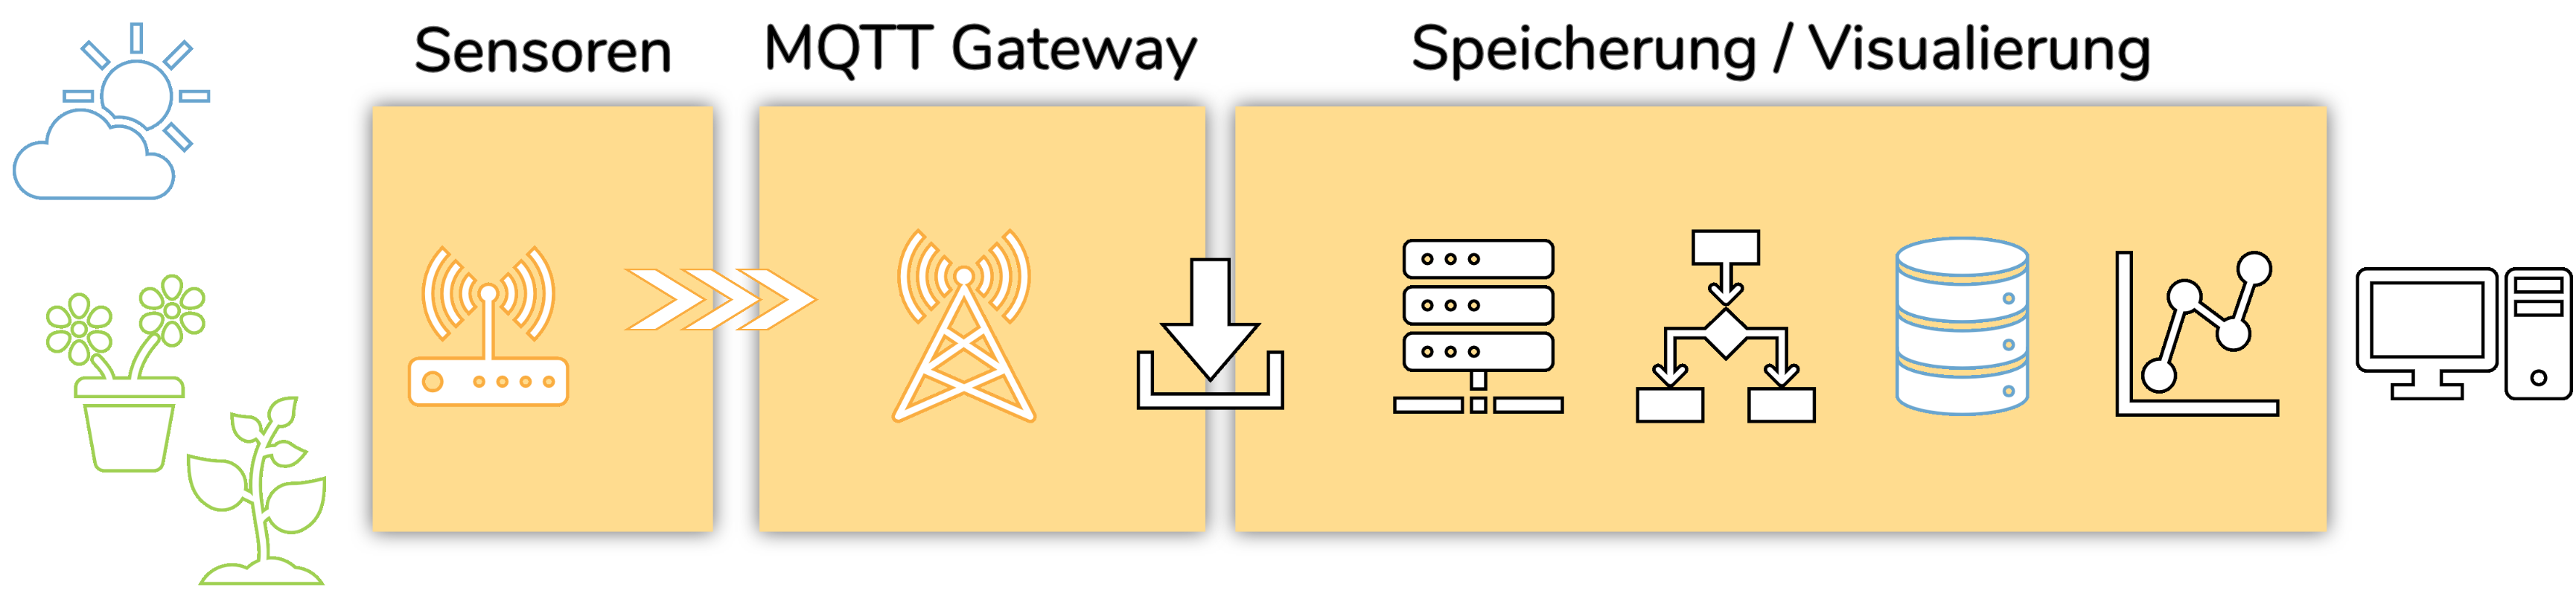
\includegraphics[width=18cm, left]{Bilder/Overview.png}
     \captionsetup{justification=centering}
      \captionof{figure}{Systemaufbau Funknetzwerk}
  \end{center}
   
Das realisierte Netzwerk besteht aus mehreren Sensoren welche Messdaten über Funk an ein MQTT-Gateway senden welches wieder über das Netzwerk mit der Datenbank verbunden ist. Für die Speicherung der Daten wird eine Zeitreihendatenbank verwendet welche speziell für die Behandlung von Messwerten optimiert ist.

  \begin{center}
    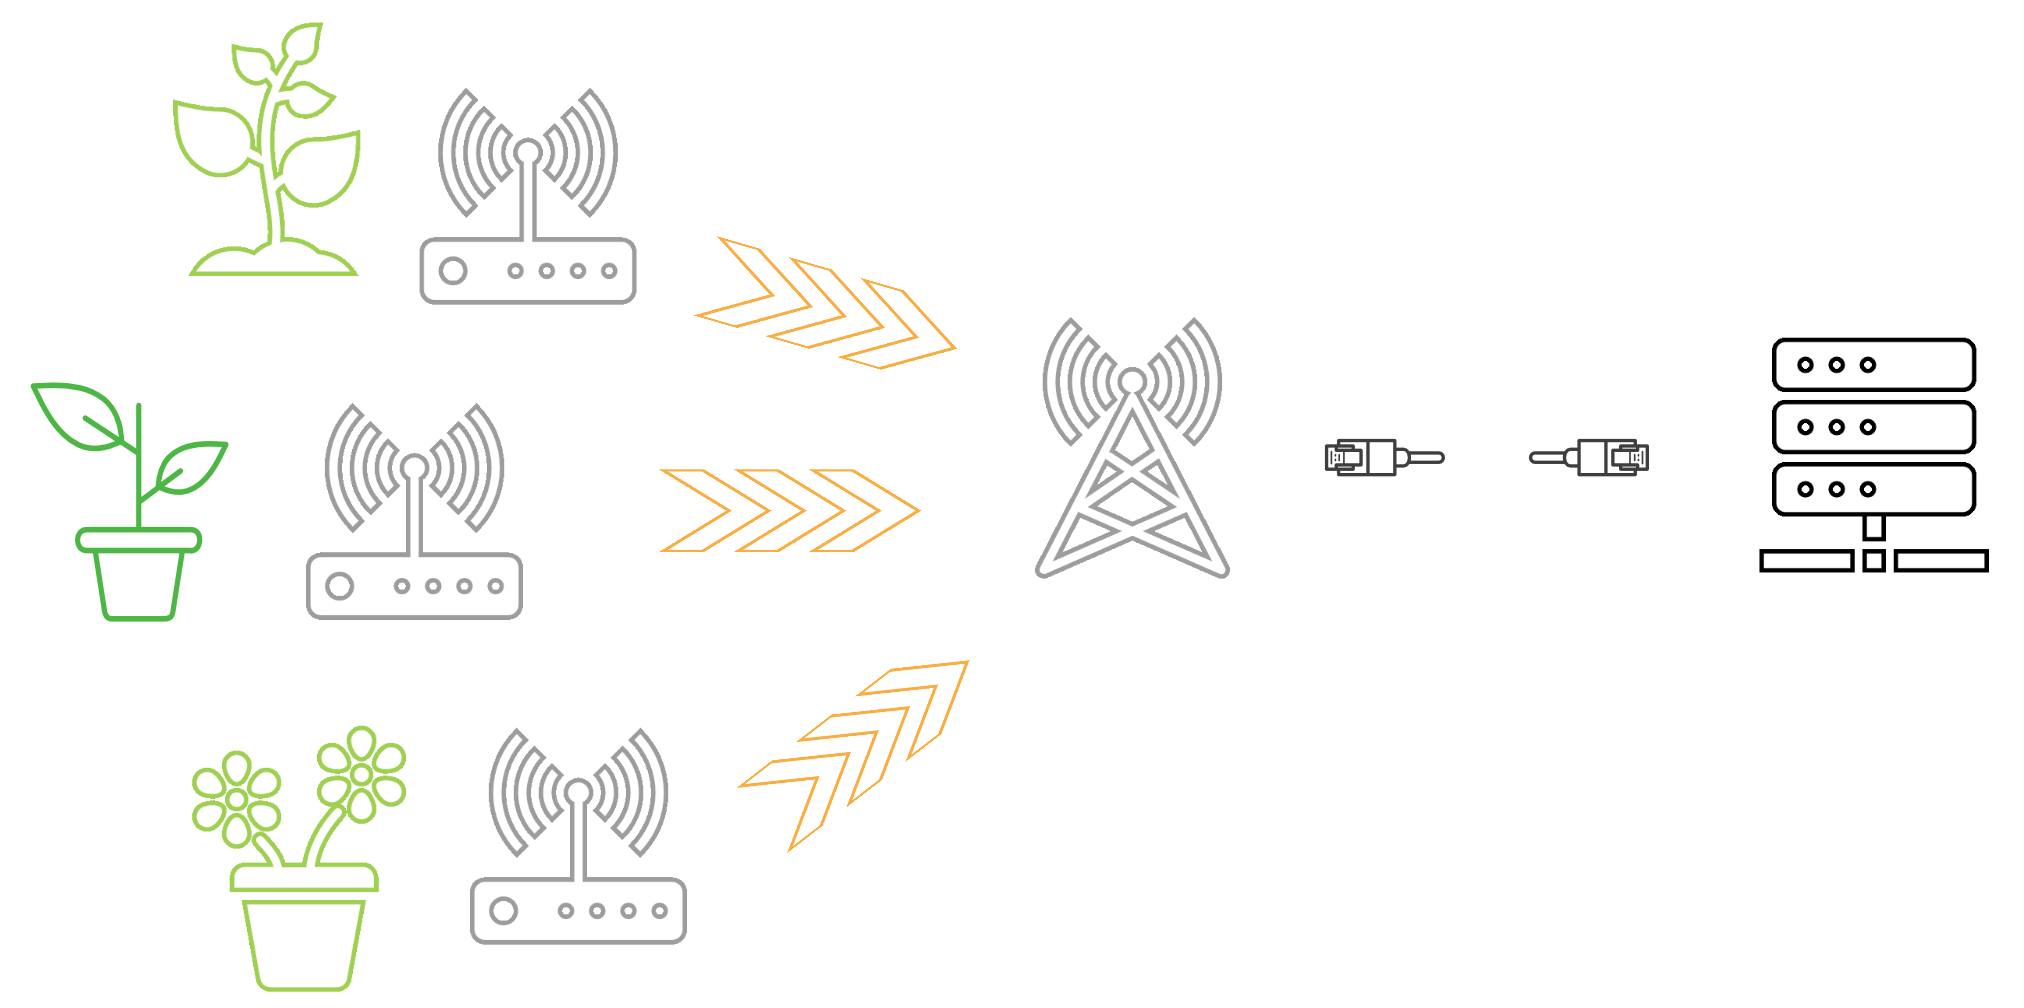
\includegraphics[width=14cm, left]{Bilder/Overview-2.png}
     \captionsetup{justification=centering}
      \captionof{figure}{Systemaufbau}
  \end{center}
  Schlussendlich werden die Daten visualisiert und können über einen Browser betrachtet werden. Beim erreichen oder unterschreiten selbst definierter Schwellwerte kann ein Alarm ausgelöst werden.
\chapter{Einleitung}
\section{Übersicht}
Die Komponenten wurden durch das Vorhandensein von Bibliotheken und Treibern sowie die leichte Beschaffung auch innerhalb der Schweiz bestimmt. Der Verzicht auf kommerzielle Systeme erlaubt eine grosse Flexibilität in der Kombination von Funktionalitäten.
\section{Hardware}

\chapter{Sensor Plattform}
\section{Mikrokontroller}
Ein sehr beliebter Mikrokontroller ist der ESP32 von Espressif \cite{espressif} welcher durch grossen Funktionsumfang und einen recht geringen Preis überzeugen kann. Ein Vorteil ist ebenfalls die Möglichkeit der Programmierung durch die Arduino\cite{arduino} IDE welche frei verfügbar ist und die Entwicklung stark vereinfacht. Es existieren viele verschiedene Mikrocontroller welche den ESP32 Baustein verwenden, für dieses Projekt kam der Firebeetle \cite{firebeetle} von DF Robot zum Einsatz.  \footnote{https://www.bastelgarage.ch/firebeetle-esp32-iot-mikrocontroller-mit-wifi}
\begin{center}
\begin{minipage}[t]{0.5\linewidth}
	\centering
	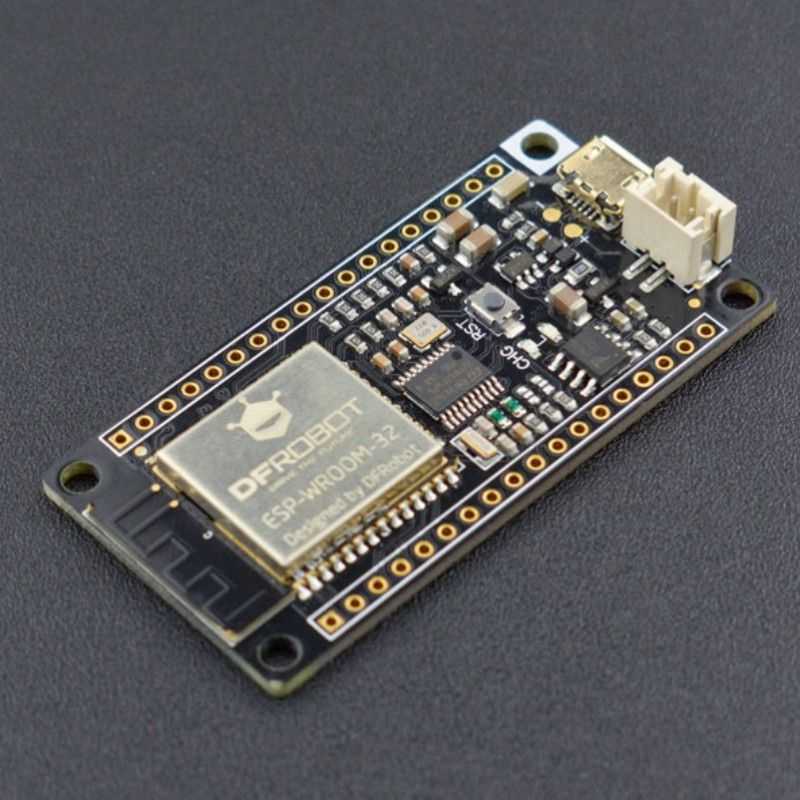
\includegraphics[ width=0.75\linewidth, valign=t]{Bilder/Firebeetle.jpg} 
	 \captionof{figure}{Firebeetle mit dem ESP32 Mikrokontroller}
\end{minipage}%
\begin{minipage}[t]{0.5\linewidth}
Der ESP32 besitzt sowohl WLAN als auch Bluetooth LE Schnittstellen. Diese wurden jedoch aus Gründen des Stromverbrauchs (WLAN) oder der Reichweite (Bluetooth LE) in diesem Projekt nicht verwendet.\break \break
 Der Firebeetle\cite{firebeetle} Baustein hat sowohl die Möglichkeit einer Stromversorgung mit 5 Volt als auch mit 3.7 Volt, womit er direkt durch Lithium-Ionen Akkus betrieben werden kann.
\end{minipage}
\end{center}
\section{Sensoren}
 Es existiert eine grosse Anzahl an verschiedenen Sensoren welche auch für Privatanwendern nutzbar sind. In diesem Projekt wurden Sensoren gewählt für welche frei verfügbare Bibliotheken in einer Version für den ESP32 vorhanden sind. Grundsätzlich wird bei den Sensoren unterschieden zwischen solchen die 
 \begin{itemize}
	 \item Digitale Werte liefern die direkt einer Einheit (Grad Celsius) oder Prozentangabe (Luftfeuchtigkeit) entsprechen
	  \item Analoge Messwerte welche auf eine Einheit umgerechnet werden müssen
\end{itemize}
Für dieses Projekt wurden mehrere Sensoren ausgewählt und kombiniert:
\begin{itemize}
	\item Lufttemperatur- und Luftfeuchtigkeitssensoren DHT11 [\ref{DHT11}] und DHT22 [\ref{DHT22}]
	\item Kapazitiver Bodenfeuchtesensor V1.2 [\ref{moistV1.2}]
\end{itemize}
\section{Aufbau}
Die Komponenten werden alle mit den 3.7 Volt und Masse Anschlüssen verbunden. Das Funkmodul benötigt die SPI Kontakte SCK, MOSI und MISO und zusätzlich zwei Digitale Pins für CE und CSN welche frei gewählt werden können. In meinem Code habe ich CE auf den Pin 25 gesetzt und CSN auf Pin 26. Wenn man andere Pins verwenden möchte dann kann dies bei Initialisierung des Funkmoduls angegeben werden: \mint{c}|radio = new RF24(25, 26); //CE, CSN|
Der Daten-Input des Temperatur Sensors benötigt einen Digitalen Eingang welchen ich auf den Pin 27 gesetzt habe. Der Bodenfeuchtigkeitssensor hat einen analogen Ausgang welchen ich mit Pin 4 verbunden hab. Falls andere Pins verwendet werden so können die Variablen am Anfang des Programms angepasst werden:
\begin{minted}{c}
// DHT Sensor
uint8_t DHTPin = 27;
// Moisture Sensor
uint8_t MOISTSENSOR_PIN = 4;
\end{minted}
Die Schaltung kann über den Mikro-USB Anschluss oder einen Lithium-Ionen-Akku mit Strom versorgt werden. Wenn ein Akku direkt angeschlossen werden soll hat es auf der Rückseite  unterhalb des USB Anschlusses zwei Lötaugen. Ein so angeschlossener Akku kann danach über die USB Buchse geladen werden, der ESP32 enthält zu diesem Zweck eine Lade-Elektronik.

  \begin{center}
    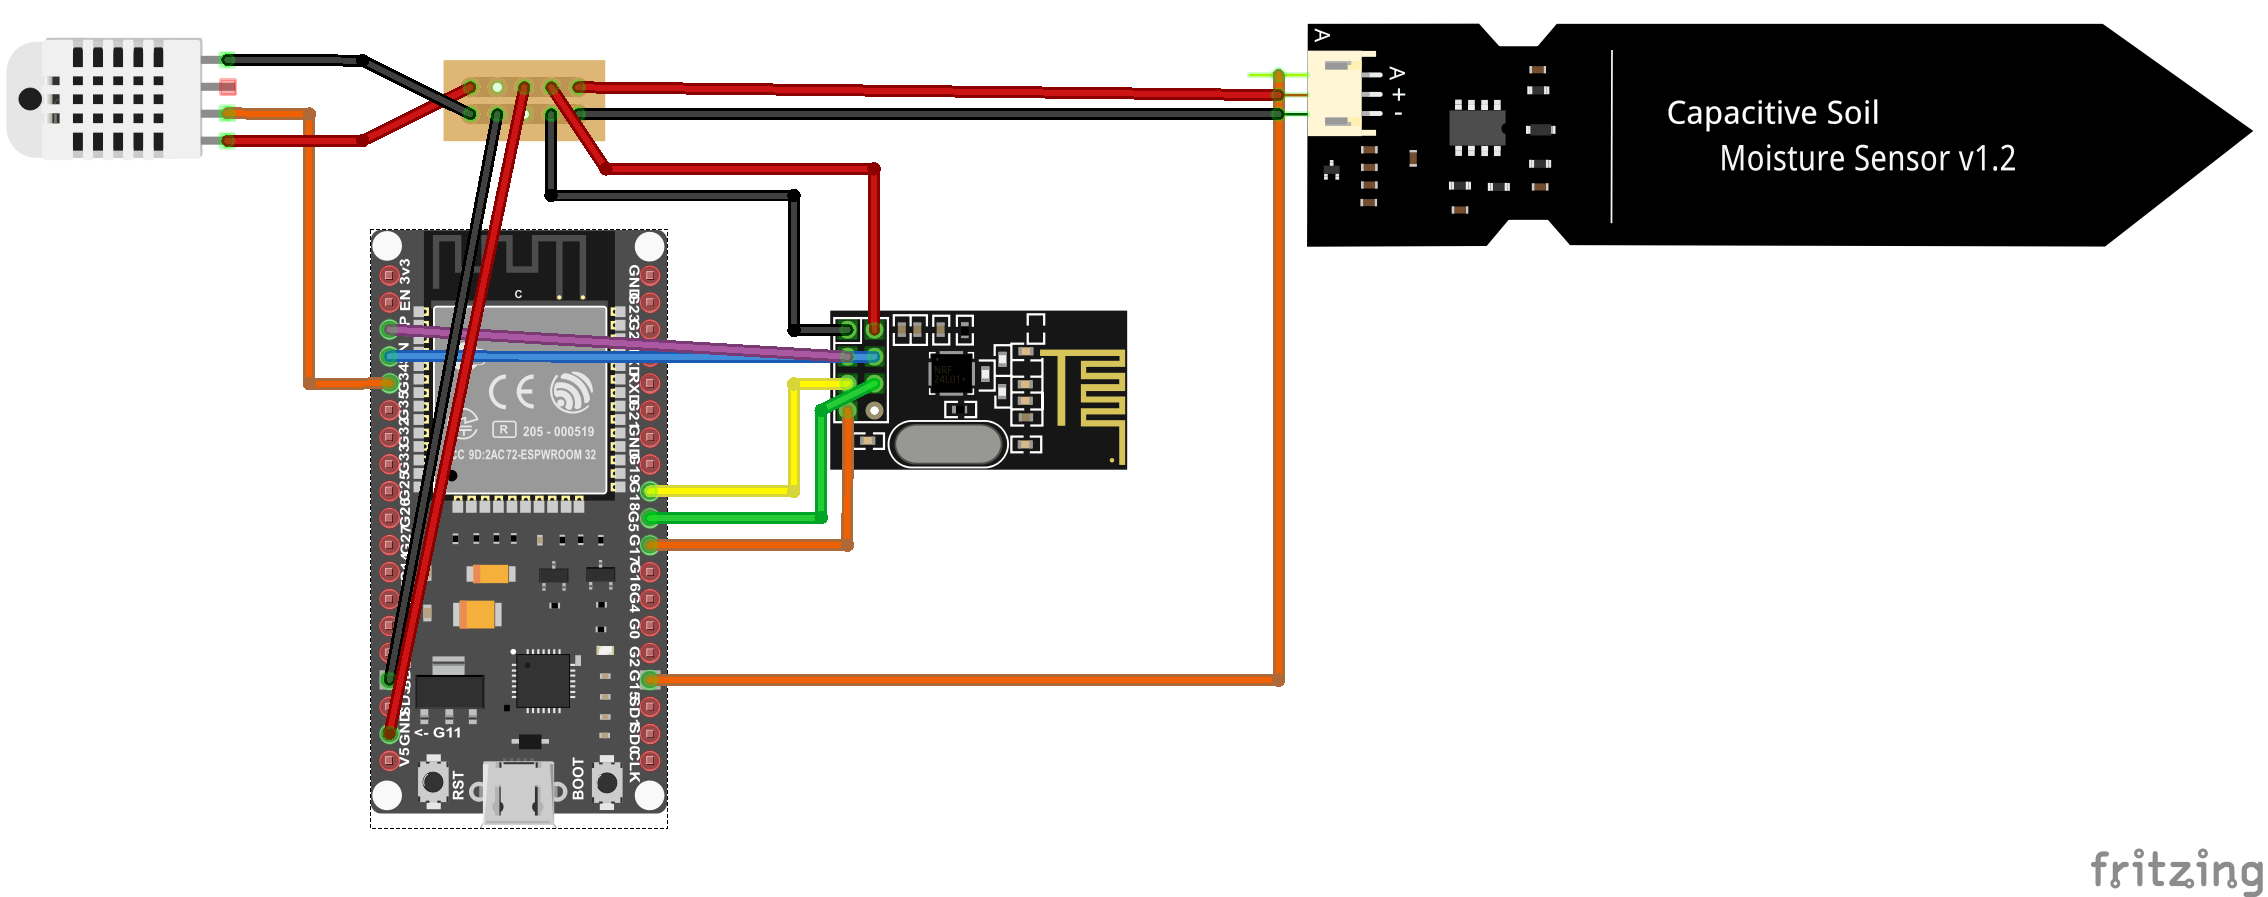
\includegraphics[width=17cm, left]{Bilder/Sensor-Design_Steckplatine.png}
    \captionsetup{justification=centering}
    \captionof{figure}{Verdrahtung der Komponenten}
   \end{center}


 \section{Funkverbindung mit dem MQTT Gateway}
 Da die Sensoren nicht WLAN als Funktechnik verwenden können sie nicht direkt auf den MQTT Server verbinden und Nachrichten senden. Diese Aufgabe übernimmt das MQTT-Gateway welches auf der einen Seite ebenfalls mit einem NRF24\ref{nrf24} Funkmodul ausgerüstet ist und andererseits eine Ethernet Netzwerkanbindung hat.
 
 Jedes Funkmodul kann mit 5 anderen Modulen kommunizieren, dabei muss jedes Modul eine eigene Adresse verwenden unter der es senden und empfangen kann.
\begin{center}
    \begin{minipage}[b]{0.45\textwidth}
        \centering
        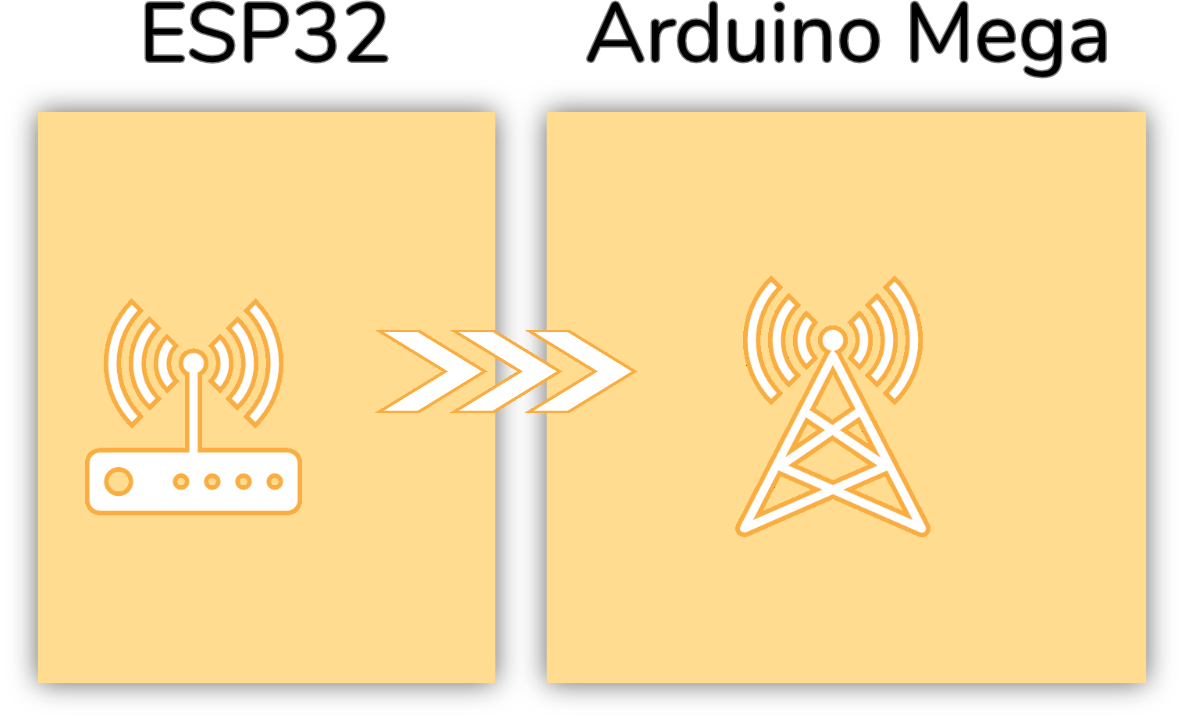
\includegraphics[width=7cm]{Bilder/ESP32-Arduino.png} % first figure itself
        \captionsetup{justification=centering}
        \captionof{figure}{Funkverbindung}
    \end{minipage}\hfill
    \begin{minipage}[b]{0.45\textwidth}\label{nrf24}
        \centering
        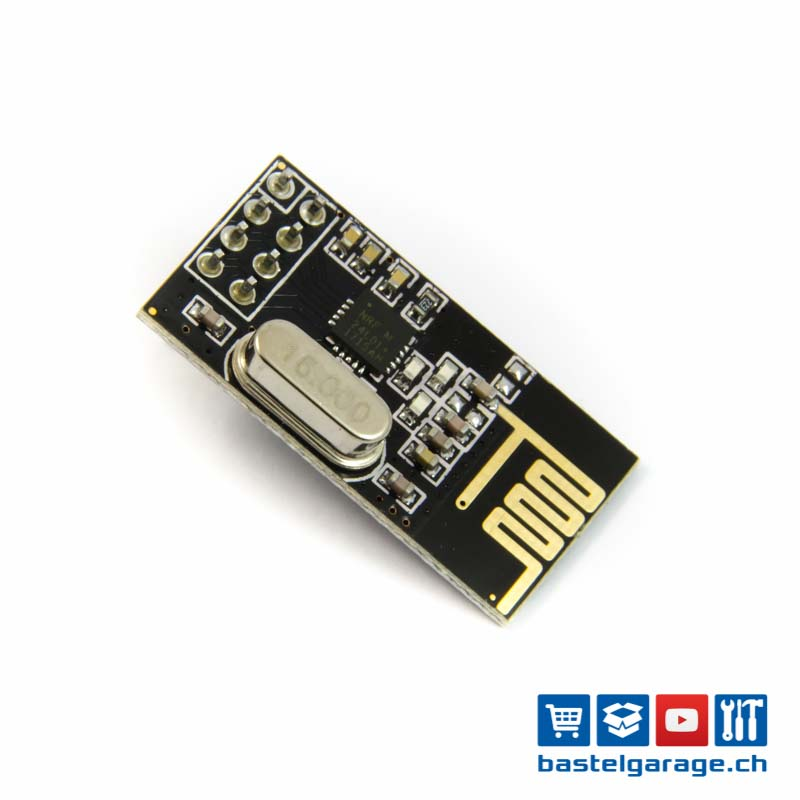
\includegraphics[width=\compImgSize]{Bilder/NRF24.jpg} % second figure itself
        \captionsetup{justification=centering}
        \captionof{figure}{NRF24L01+ Funkmodul}
    \end{minipage}
\end{center}
Bei der Programmierung der Sensoren wurde darauf geachtet dass die Identifikation der Sensoren über eine einzigartige Id unabhängig vom Programmcode vorgenommen werden kann [\ref{config}].
\begin{center}
    \begin{minipage}[b]{0.45\textwidth}
        \centering
        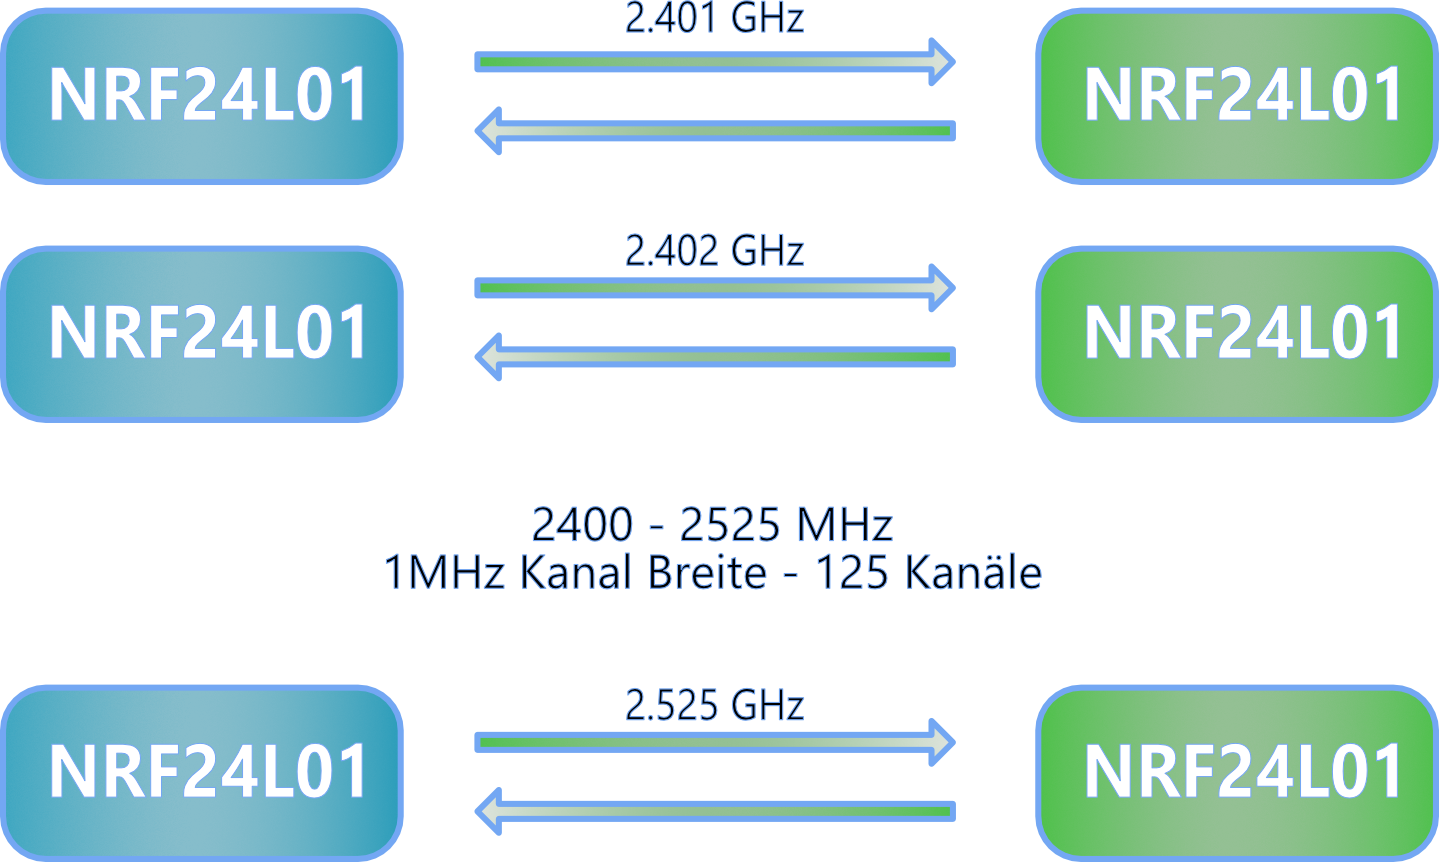
\includegraphics[width=9cm]{Bilder/NRF24Kommunikation.png}
        \captionsetup{justification=centering}
        \captionof{figure}{Funkkanäle des NRF24L01}
    \end{minipage}\hfill
    \begin{minipage}[b]{0.45\textwidth}
        \centering
        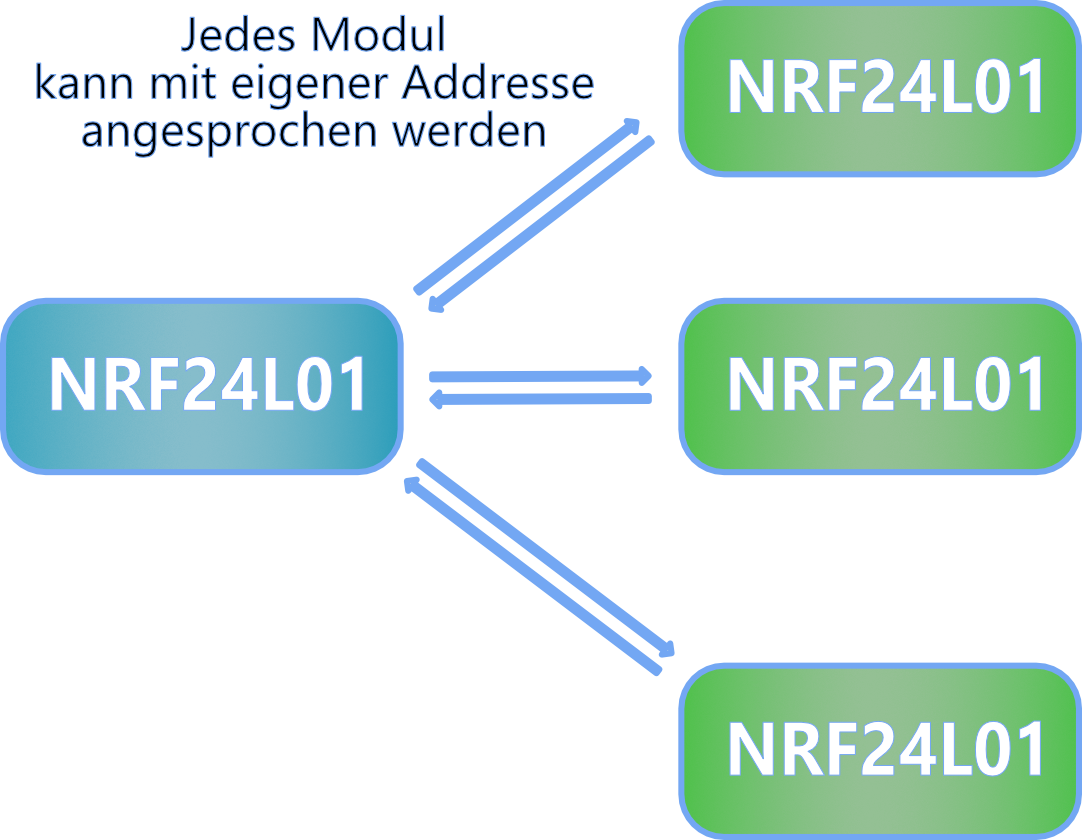
\includegraphics[width=7cm]{Bilder/NRF24Kommunikation-2.png} % second figure itself
        \captionsetup{justification=centering}
        \captionof{figure}{Addressierung Funkmodule}
    \end{minipage}
\end{center}
\subsection{Absicherung der Funkverbindung}
Die Identifikation eines Sensors ist aber nicht zu Verwechseln mit einer Prüfung ob der Sender überhaupt berechtigt ist Daten zu senden. Da das Funkprotokoll unverschlüsselt ist können andere Sender ebenfalls Nachrichten absenden und so Daten verfälschen oder die Verarbeitung stören. Um dies zu verhindern wird eine Technik Namens \Gls{hmac} eingesetzt.
Die eigentliche Nachricht \mint{html}| 4;25.1;71.1;10.2| wird dabei um einen Hash-Wert erweitert
\mint{html}|3A51266ABD432C1FB797DEDEE215FD16E42BAB627F104BCB6F4169EDE4544582:4;25.1;71.1;10.2|

 \section{Software}
 \subsection{Verwendete Bibliotheken}

  \begin{description}
\item[SPI library] Ansteuerung der Sensoren \cite{spi}
\item[mbed TLS] Berechnung des \Gls{hmac} \cite{mbedTLS}
\item[RF24] Funkmodul \cite{nrf24}
\item[DHT-sensor-library] Luft- und Feuchtigkeitssensor \cite{dht}
 \end{description}
Einige der aufgeführten Bibliotheken können direkt über die Bibliotheksverwaltung der Arduino IDE installiert werden. Ansonsten können die Bibliotheken über den Link (führt meistens auf github.com) heruntergeladen und von Hand installiert werden. 
{\color{red}Achtung: Es gibt viele Bibliotheken mit ähnlichem Namen und Beschreibung. Falls das kompilieren fehlschlägt bitte prüfen ob die richtige Bibliothek eingebunden wurde.}

 \subsection{Konfiguration eines Sensors}\label{config}
\begin{center}
    \begin{minipage}[b]{0.45\textwidth}
       Der Flash-Speicher des ESP32 kann in mehrere Bereiche unterteilt werden. So können Dateien unabhängig von dem kompilierten Programm auf den Mikrocontroller geladen werden. Während der Programm-Code während der Entwicklung ständig ändert und immer wieder via Sketch-Upload auf den ESP32 übertragen werden so müssen die Konfigurationsparameter nur einmal festgelegt werden und ändern sich, wenn überhaupt, nur selten.
 \break
 \break
      \begin{forest}
	    for tree={font=\sffamily, grow'=0,
	    folder indent=.9em, folder icons,
	    edge=densely dotted}
       [FB{\_}DHT11{\_}NRF24
	    	[FB{\_}DHT11{\_}NRF24.ino, is file]
	    	[Settings.h, is file]
		      [data, this folder size=15pt
		          [id.txt, is file]
		          [key, is file]
		          [settings.txt, is file]
			]
	    ]
	  \end{forest}
	  \captionof{figure}{Verzeichnisstruktur Sensor}
    \end{minipage}\hfill
    \begin{minipage}[b]{0.45\textwidth}
    \raisebox{\dimexpr-\height+\ht\strutbox\relax}{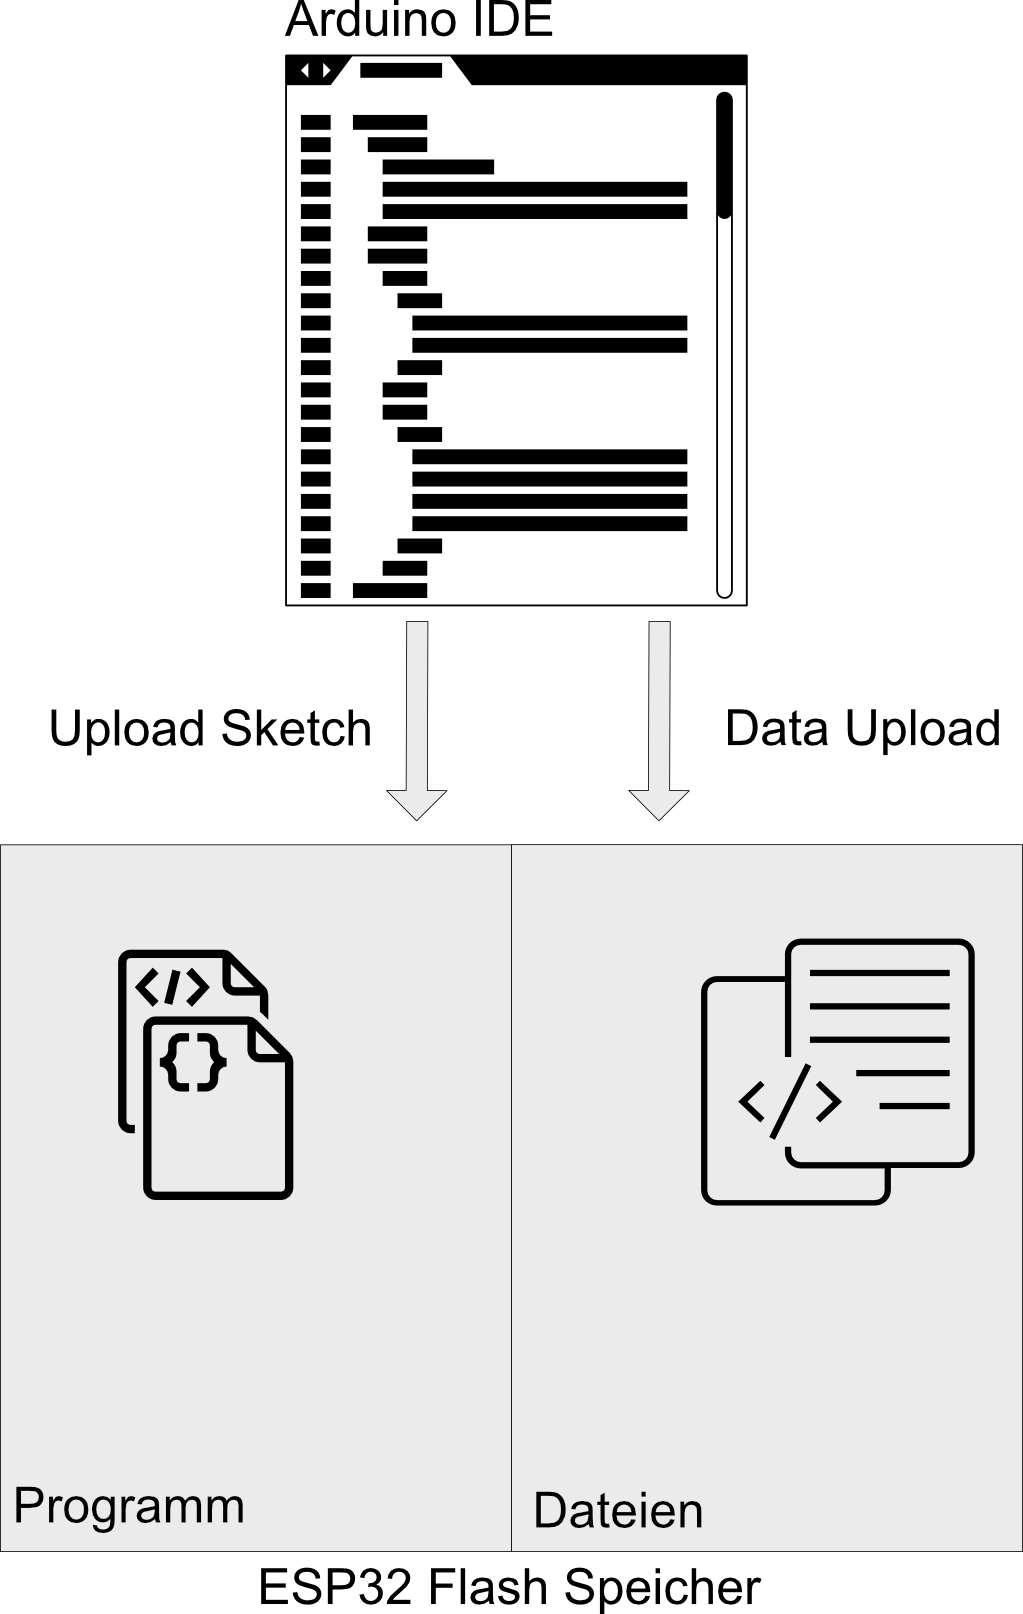
\includegraphics[width=7cm, left]{Bilder/ESP32-Memory-Organisation.png}}
    \captionsetup{justification=centering}
    \captionof{figure}{Speicher-Aufteilung ESP32}
	\end{minipage}
\end{center}

 Jeder Sensor benötigt einige Parameter:
 \begin{description}
\item[Id] Identifiziert den Sensor, gespeichert in der Datei id.txt
\item[key] Der geheime Schlüssel um den \Gls{hmac} zu berechnen, gespeichert in der Datei key. Dieser Schlüssel muss auf den Sensoren wie auf dem Gateway identisch sein.
\end{description}
Die folgende Parameter werden alle in der Datei settings.txt gespeichert:
 \begin{description}
\item[sensorType] Typ des Temperatursensor, entweder DHT11 oder DHT22
\item[sleepTime] Wartezeit zwischen zwei Messungen in Millisekunden
\item[paLevel] Funkstärke des NRF24 Moduls, erlaubte Werte sind 'low', 'med und 'high'
\end{description}
%
\chapter{IoT Gateway}
\section{Übersicht}
\section{Hardware}
\section{Funkverbindung}
\subsection{Aufbau}
\begin{center}
  \begin{center}
    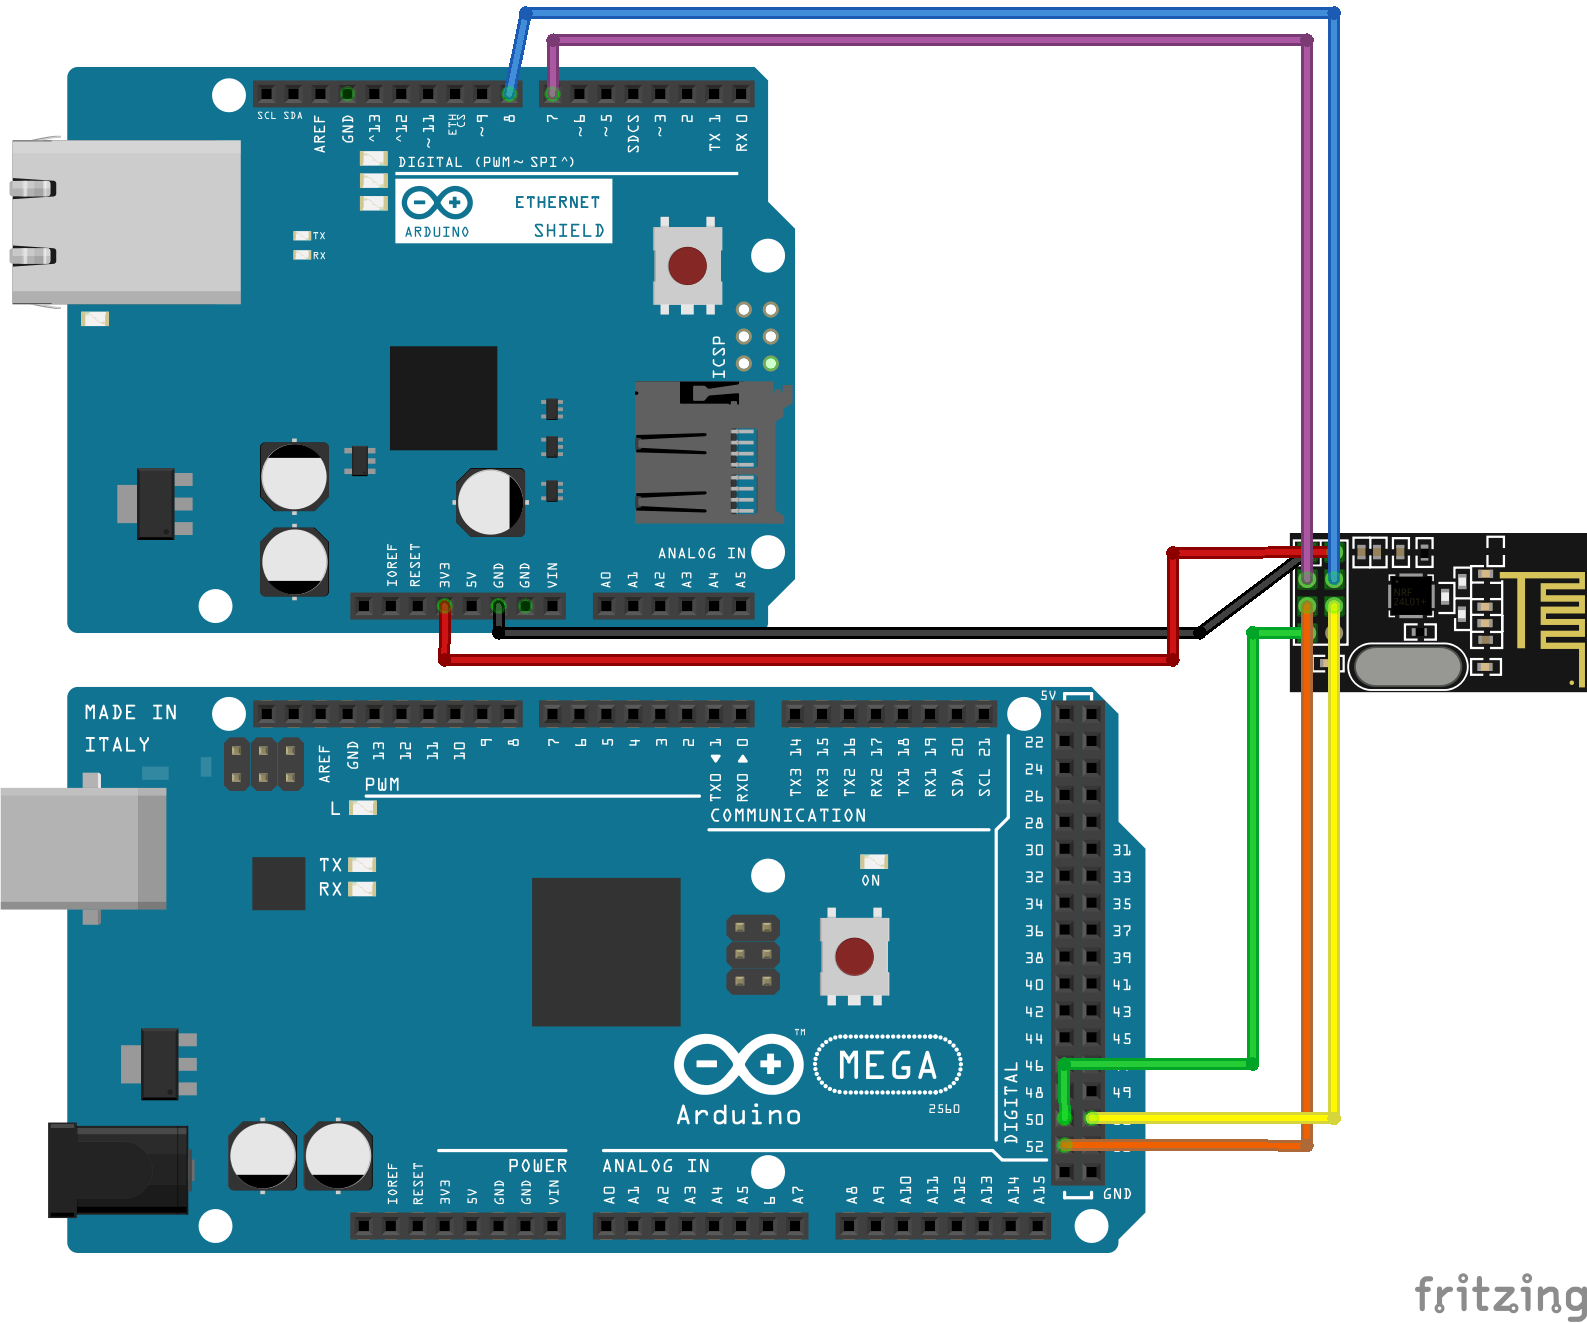
\includegraphics[width=12cm, left]{Bilder/MQTT-Gateway-Design_Steckplatine.png}
  \end{center}
    \captionof{figure}{Verdrahtung der Komponenten}
\end{center}
\subsection{Zugriffsschutz}
Jede empfangene Nachricht wird durch die Valdierung des HMAC (\Gls{hmac}) sowohl auf einen berechtigten Absender, als auch auf unverfälschte Daten überprüft.
\section{Software}
\subsection{Konfiguration}
Das Gateway benötigt für die Berechnung des \Gls{HMAC} den gleichen Schlüssel wie der Sensor. Leider bietet der Arduino nicht die Möglichkeit Dateien hochzuladen. Der benötigte geheime Schlüssel wird deshalb in der Datei keyFile.h als String definiert. So kann der Code weiterhin in dem Versionskontrollsystem hinterlegt werden ohne den geheimen Schlüssel preisgeben zu müssen.
\begin{center}
    \begin{minipage}[b]{0.45\textwidth}
    	Die Datei keyFile.h enthält nur eine Zeile mit der Deklaration des Schlüssels \mint{html}|String key_str  = "geheimerSchlüssel";|
    \end{minipage}\hfill
    \begin{minipage}[b]{0.45\textwidth}
	\begin{forest}
		    for tree={font=\sffamily, grow'=0,
		    folder indent=.9em, folder icons,
		    edge=densely dotted}
	       [Arduino{\_}NRF24{\_}Receiver
		    	[Arduino{\_}NRF24{\_}Receiver.ino, is file]
		    	[keyFile.h, is file]
		    ]
	\end{forest}
	\end{minipage}
\end{center}

\begin{listing}
\begin{minted}{js}
{     
    "ID": 0001, 
    "Temp.Air": 22.6,
    "Hum.Air": 78.1, 
    "Hum.Soil": 43.7
}
\end{minted}
\caption{Sensor Datensatz in JSON Format} 
\label{json-example}
\end{listing}

\chapter{Speicherung und Visualisierung}
\section{Übersicht}
Für die Speicherung und Verarbeitung der gesammelten Sensordaten sind mehrere Softwarekomponenten zuständig.
\begin{center}
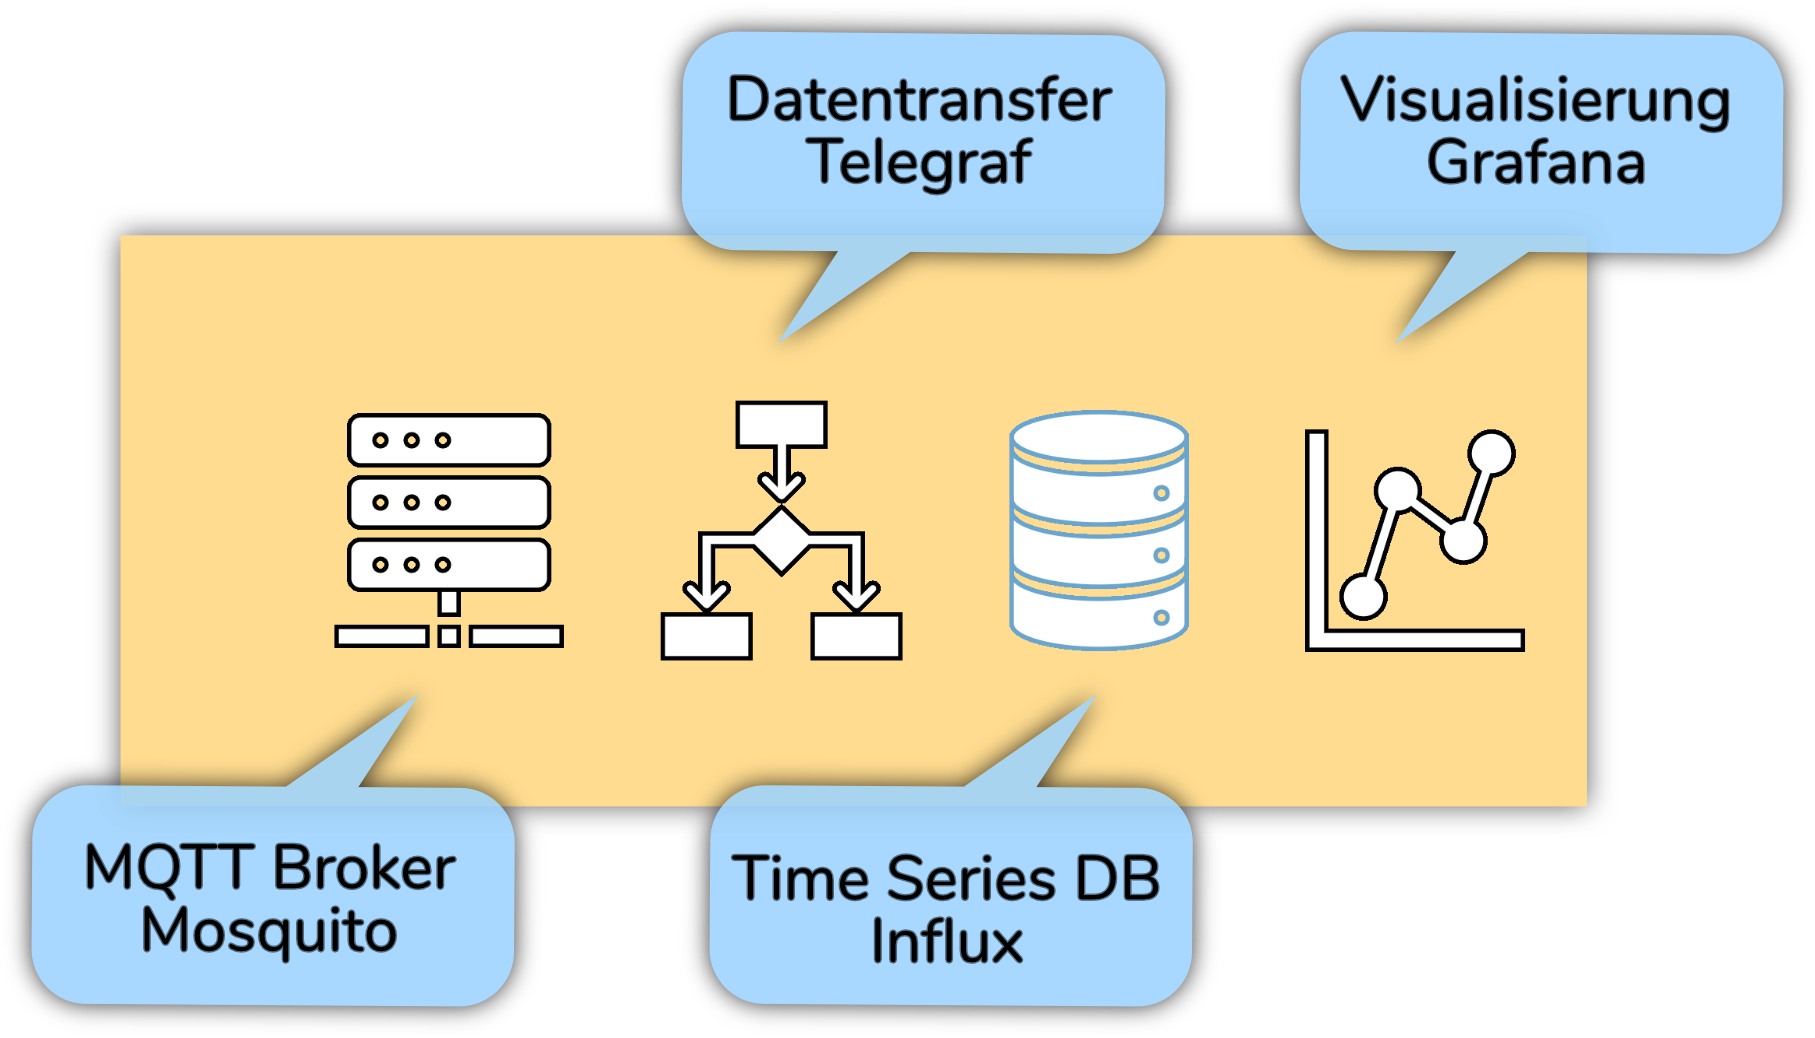
\includegraphics[width=17cm, left]{Bilder/Raspberry-Software.png}%
\captionof{figure}{Verwendete Software}\label{labelname}%
\end{center}
 \begin{description}
\item[MQTT Broker] Die von dem MQTT-Gateway geschickten Nachrichten werden durch Mosquitto \cite{mosquitto} in einer Queue bis zu einer weiteren Verarbeitung gespeichert
\item[Datentransfer] Um die Daten aus einer (oder mehreren) MQTT Queue in eine Datenbank zu transferieren wird Telegraf \cite{telegraf} mit dem MQTT Plugin benutzt \cite{telegrafmqtt}
\end{description}
\section{Hardware}
\section{MQTT Broker}
\subsection{Installation}
\begin{minted}{Bash}
sudo apt-get install -y mosquitto mosquitto-clients
   \end{minted}
\section{Datenspeicherung}
  \begin{center}
    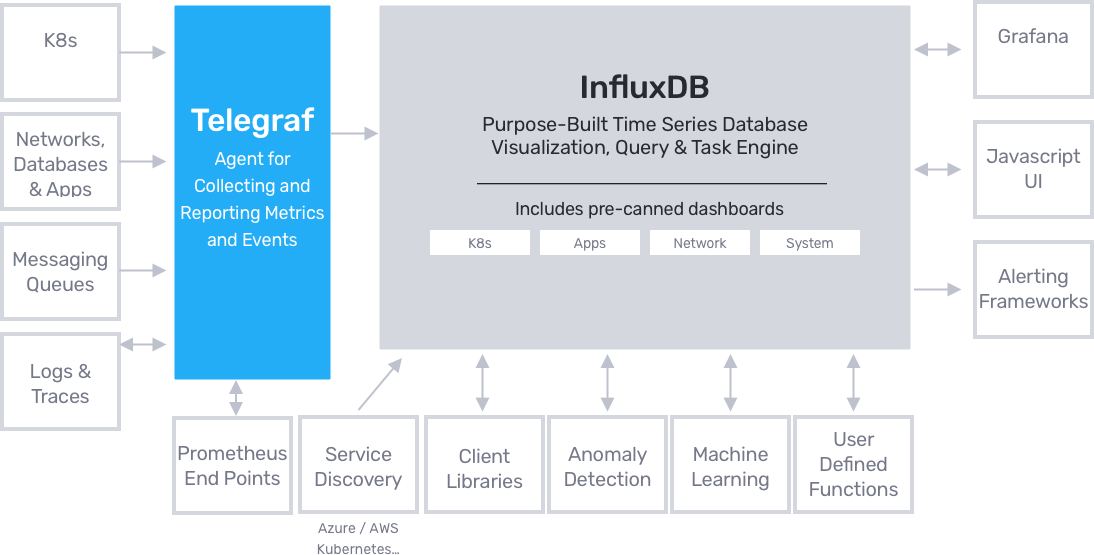
\includegraphics[width=\textwidth]{Bilder/InfluxDB-2.png}
    \captionsetup{justification=centering}
    \captionof{figure}{Übersicht Influx Software}
    \source{\url{www.influxdata.com}}
   \end{center}
   \subsection{Installation}
   Die Installationsquelle ist unterschiedlich für die verschiedenen Linux Distributionen. Wenn wie in meinem Fall die Raspian Distribution in der Version 'buster' verwendet wird kann das benötigte Repository mit folgenden Kommandos hinzugefügt werden:
 \begin{minted}[breaklines]{Bash}
curl -sL https://repos.influxdata.com/influxdb.key | sudo apt-key add -
sudo apt install apt-transport-https
echo "deb https://repos.influxdata.com/debian buster stable" | sudo tee /etc/apt/sources.list.d/influxdb.list
\end{minted}
Die Installation ist danach schnell gemacht:
 \begin{minted}{Bash}
sudo apt-get update && sudo apt-get install influxdb
sudo systemctl unmask influxdb.service
   \end{minted}
   Danach muss der Service noch gestartet werden:
    \begin{minted}{Bash}
sudo systemctl start influxdb
   \end{minted}
   \subsection{Datenbank einrichten}
   
\section{Visualisierung}
\subsection{Installation}
    \begin{minted}[breaklines]{Bash}
wget https://github.com/fg2it/grafana-on-raspberry/releases/download/v5.1.4/grafana_5.1.4_armhf.deb
sudo apt-get install -y adduser libfontconfig1
sudo dpkg -i grafana_5.1.4_armhf.deb
sudo systemctl enable grafana-server
sudo systemctl start grafana-server
sudo systemctl enable grafana-server.service
   \end{minted}
\chapter{Verwendete Bauteile}
\section{ESP32 Mikrokontroller}
\begin{center}
    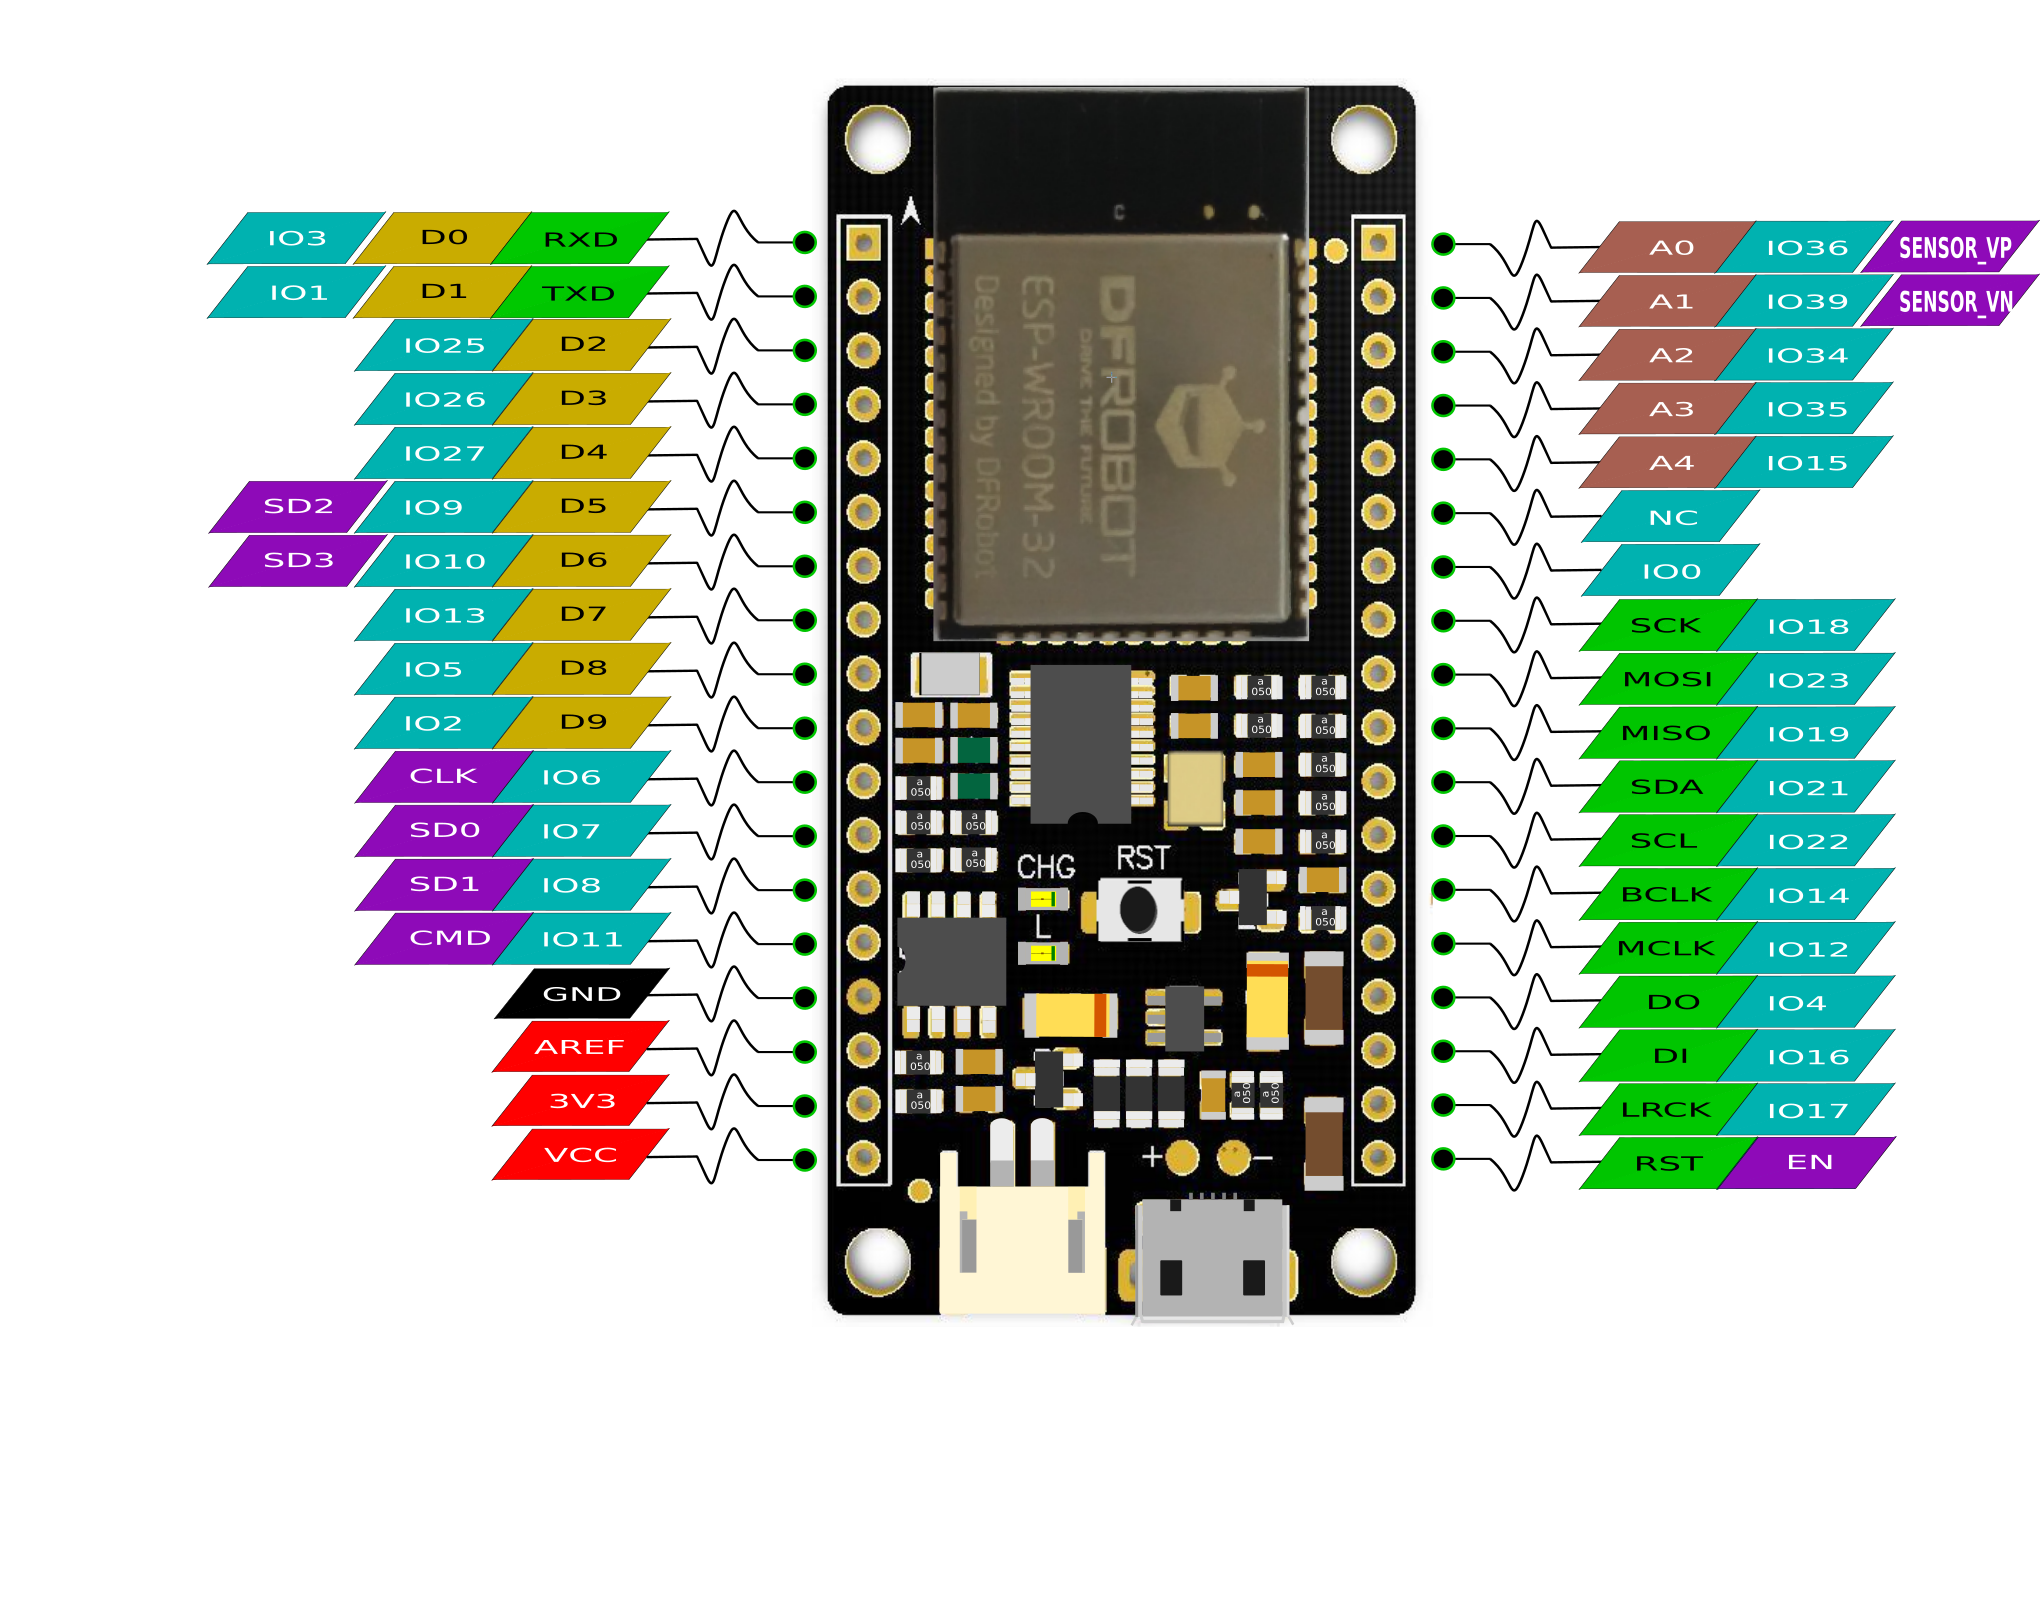
\includegraphics[width=14cm, left]{Bilder/FireBeetleBoard.png}
    \captionsetup{justification=raggedright}
    \captionof{figure}{Anschlüsse des Firebeetle}
\end{center}
 \section{Sensoren}
 \subsection{Temperatur und Luftfeuchtigkeit}
 \subsubsection{DHT22}\label{DHT22}
\begin{flushleft}
	\begin{minipage}[t]{0.5\linewidth}
		\centering
    		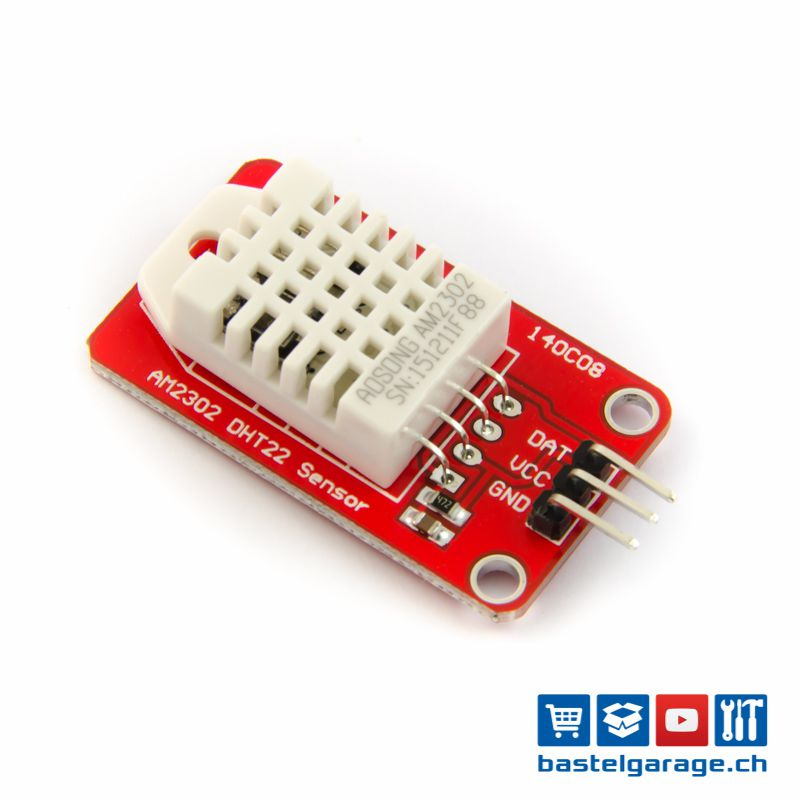
\includegraphics[width=\compImgSize, left]{Bilder/DHT22.jpg}
    		\captionof{figure}{Temperatur und Luftfeuchtigkeitsmesser DHT22}
	\end{minipage}%
	\begin{minipage}[t]{0.5\linewidth}
	DHT22 im Onlineshop \footnotemark
	\end{minipage}
	\footnotetext{https://www.bastelgarage.ch/dht22-temperatur-und-luftfeuchtigkeitssensor-steckbar}
\end{flushleft}

\subsubsection{DHT11}\label{DHT11}
\begin{flushleft}
	\begin{minipage}[t]{0.5\linewidth}
		\centering
		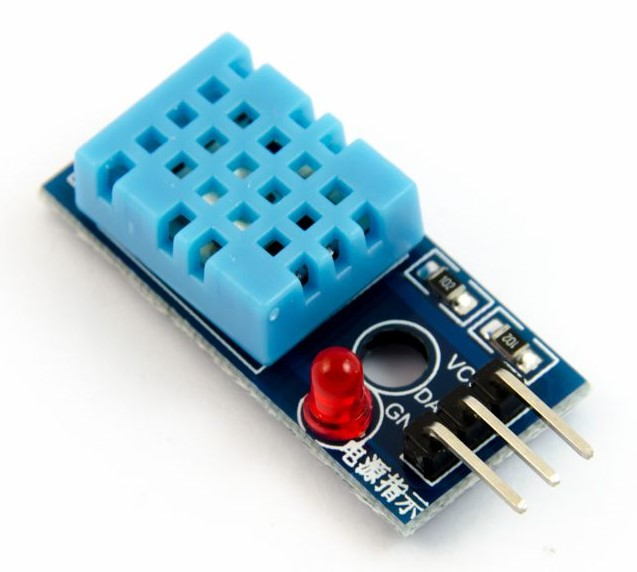
\includegraphics[ width=\compImgSize, left]{Bilder/DHT11.jpg} 
		 \captionof{figure}{DHT11 Luft- und Feuchtigkeitssensor}
	\end{minipage}%
	\begin{minipage}[t]{0.5\linewidth}
	Als Alternative zu dem oben genannten DHT22 gibt es eine billigere Variante mit dem Namen DHT11 \footnotemark.
	Der DHT11 Sensor hat eine geringere Auflösung als der DHT22, ist ansonsten aber gleich verwendbar.
	\end{minipage}
	 \footnotetext{https://www.bastelgarage.ch/dht11-temperatur-und-luftfeuchtigkeitssensor}
\end{flushleft}

\subsection{Bodenfeuchtigkeit}\label{moistV1.2}
\begin{center}
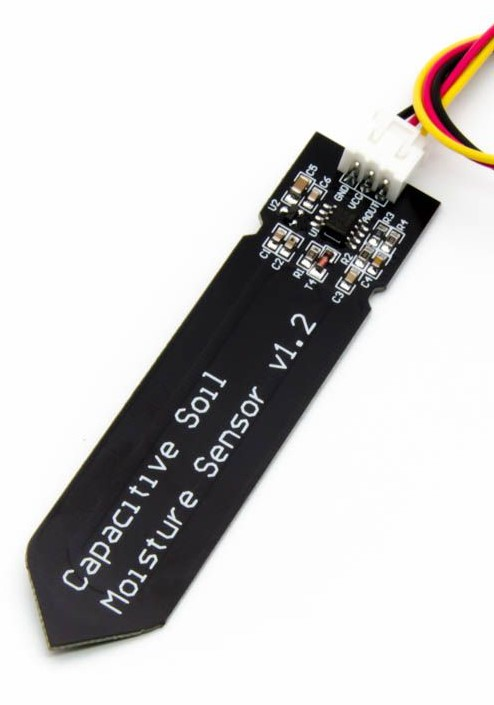
\includegraphics[width=\compImgSize, left]{Bilder/Soil-2.jpg}%
\captionof{figure}{Kapazitiver Bodenfeuchtesensor V1.2}\label{labelname}%
\end{center}
Bodensensor im Onlineshop \footnote{https://www.bastelgarage.ch/bauteile/sensoren/kapazitiver-bodenfeuchtesensor-v1-2}
\subsection{Funk}
\begin{flushleft}
        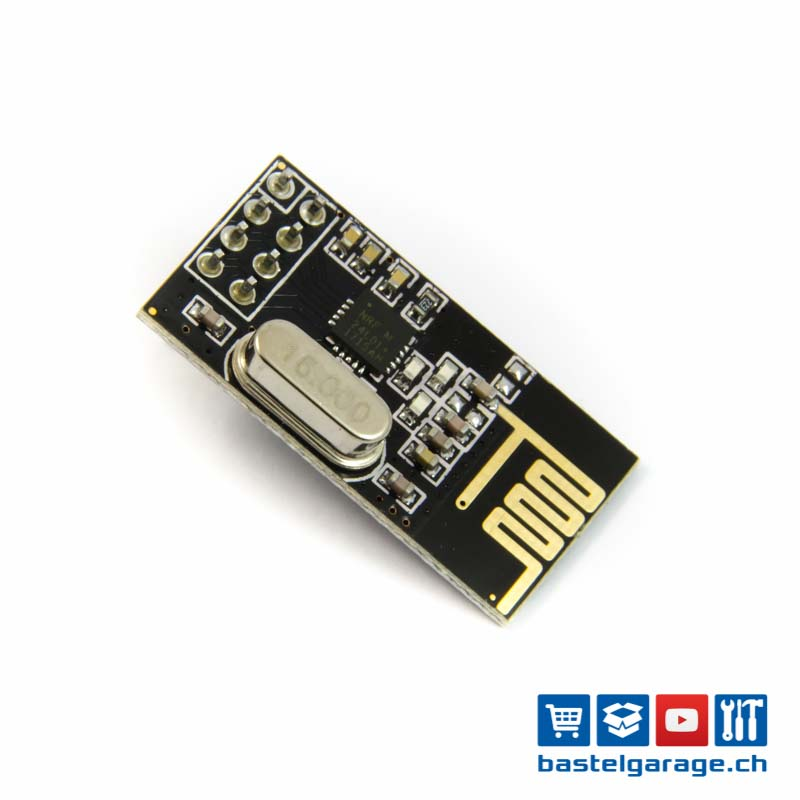
\includegraphics[width=\compImgSize]{Bilder/NRF24.jpg} % second figure itself
        \captionsetup{justification=raggedright}
        \captionof{figure}{NRF24L01+ Funkmodul}
\end{flushleft}
NRF24L01+ \footnote{https://www.bastelgarage.ch/bauteile/funk-wireless-lora/nrf24l01-wireless-funk-modul-2-4ghz}
% List of Figures
\listoffigures
% List of Tables
\listoftables
% Glossary
\printglossary
% Bibliography

\renewcommand\bibname{Linkverzeichnis}
\begin{thebibliography}{99}
   \bibitem{whyHmac}What is HMAC Authentication and why is it useful?\break \url{https://www.wolfe.id.au/2012/10/20/what-is-hmac-authentication-and-why-is-it-useful/}
    \bibitem{esp32-hmac}ESP32 Arduino: Applying the HMAC SHA-256 mechanism\break \url{https://techtutorialsx.com/2018/01/25/esp32-arduino-applying-the-hmac-sha-256-mechanism/}
    \bibitem{mbedTLS} mbed TLS, Library für den ESP32 welche viele Kryptografische Funktionen implementiert\break \url{https://tls.mbed.org/}
    \bibitem{spi} Standard Bibliothek sowohl für den Arduino wie auch den ESP32 welche die Kommunikation mit anderen Komponenten, in diesem Fall die einzelnen Sensor Module, übernimmt\break \url{https://www.arduino.cc/en/Reference/SPI}
    \bibitem{rfh24} Bibliothek für den nRF24L01 Baustein welche sowohl auf dem Arduino als auch dem ESP32 verwendbar ist \break \url{https://github.com/nRF24/RF24}
    \bibitem{hmacOnline}Online HMAC Code Generator\break \url{https://www.freeformatter.com/hmac-generator.html#ad-output}
    \bibitem{nrf24}NRF24L01+ Funkmodul Treiber für Arduino und ESP32\break \url{http://tmrh20.github.io/RF24/index.html}
    \bibitem{dht} Bibliothek für die beiden Sensoren DHT11 und DHT22 sowohl für Arduino als auch den ESP32 \break \url{https://github.com/adafruit/DHT-sensor-library}
    \bibitem{espressif}Herstellerseite Espressif für den ESP32\break \url{https://www.espressif.com/en/products/hardware/esp32/overview}
    \bibitem{arduino}Arduino Herstellerseite mit der gleichnamigen IDE und vielen Bibliotheken und Tutorials\break \url{https://www.arduino.cc/}
    \bibitem{firebeetle}Herstellerseite des Firebeetle Mikrokontrollers\break \url{https://www.dfrobot.com/product-1590.html}
    \bibitem{uploader}Erweiterung für die Arduino IDE um Dateien in den Flash Speicher des ESP32 zu laden \break \url{https://github.com/me-no-dev/arduino-esp32fs-plugin}
    \bibitem{mosquitto}Open Source MQTT Broker Mosquitto\break \url{https://mosquitto.org/}
    \bibitem{telegraf} Server Agent welcher Daten aus verschiedenen Quellen sammelt und weiterleitet \break \url{https://www.influxdata.com/time-series-platform/telegraf/}
    \bibitem{telegrafmqtt}MQTT Plugin für Telegraf\break \url{https://github.com/influxdata/telegraf/tree/master/plugins/inputs/mqtt_consumer}
    \bibitem{influx} InfluxDB, Open Source Zeitreihendatenbank \break \url{https://www.influxdata.com/products/influxdb-overview/}
    \bibitem{grafana} Datenvisualierungs-Software Grafana\break \url{https://grafana.com/}
  \end{thebibliography}
%Index
\addcontentsline{toc}{chapter}{Index}
%\printindex
% Appendices
\end{document}
